\documentclass[aspectratio=169]{beamer}
%\documentclass[aspectratio=43]{beamer}
\usepackage [italian]{babel}
\usepackage [utf8]{inputenc}
\usepackage [T1]{fontenc}




\title [Tesi di laurea in Scienze Biologiche]{Modellazione formale applicata ad analisi \emph{in silico} di reti metaboliche}
\author [{\bfseries Lorello} Luca Salvatore] {Luca Salvatore Lorello}
\date [A.A. \bfseries{17/18}] {Anno Accademico 2017--2018}
\institute [{\bfseries DiSB}@UniUrb]{Dipartimento di Scienze Biomolecolari, Universit\`a degli Studi "Carlo Bo" di Urbino}
%\logo{
\includegraphics{alto.png}}
\usetheme {AnnArbor}

\theoremstyle {definition}
\newtheorem {definizione}{Definizione}
\theoremstyle {plain}
\newtheorem {teorema}{Teorema}


\usepackage{graphbox}
\usepackage{tabularx}
\usepackage{tikz}
\usepackage{amsfonts,
	amstext,
	amssymb,
	mathrsfs,
	pgfplots,
	pgfplotstable,
	mathtools}
\usepackage{cancel}

\usetikzlibrary{positioning}
\usetikzlibrary{pgfplots.groupplots,spy,backgrounds,shadows}

\definecolor{a}{HTML}{FCD826}
\definecolor{b}{HTML}{333399}
\definecolor{c}{HTML}{808080}
\definecolor{w}{HTML}{FFFFFF}

\setbeamercolor*{palette quaternary}{bg=a}
\setbeamercolor*{palette tertiary}{bg=a}
\setbeamercolor*{palette secondary}{bg=a}
\setbeamercolor*{palette primary}{bg=b}
\setbeamercolor*{institute in head/foot}{fg=w,bg=b}
\setbeamercolor*{page number in head/foot}{fg=w}

\newsavebox\altobox
\newsavebox\bassobox




\setbeamertemplate{headline}{%
			\sbox{\altobox}{
\includegraphics[scale=0.5]{alto.png}}
	\leavevmode%
	\hbox{%
		
\includegraphics[height=\ht\altobox]{alto.png}\hfill
		\begin{beamercolorbox}[wd=.7\paperwidth,ht=\ht\altobox,dp={0pt},sep={1ex},left]{section in head/foot}%
			{\usebeamerfont{title in head/foot}{\bfseries\inserttitle}\par
			\usebeamerfont{section in head/foot}\insertsection\phantom{pippo}}
			\vskip0pt plus 1filll
		\end{beamercolorbox}%
		\begin{beamercolorbox}[wd=.3\paperwidth,ht=\ht\altobox,dp={0pt},sep={2ex},left]{institute in head/foot}%
			\usebeamerfont{institute in head/foot}\usebeamercolor[fg]{institute in head/foot}\insertshortinstitute
%			\vskip0pt plus 1filll
		\end{beamercolorbox}}%
		\hskip0pt
		\hrule
		{\color{c}\hrule height 2pt\hfill}
		\hrule
	}

\setbeamertemplate{footline}{%
	\sbox{\bassobox}{
\includegraphics[scale=0.5]{basso.png}}
	\leavevmode%
			\hrule
			{\color{c}\hrule height 2pt\hfill}
			\hrule
	\hbox{%
		
\includegraphics[height=\ht\bassobox]{basso.png}\hfill
		\begin{beamercolorbox}[wd=.7\paperwidth,ht=\ht\bassobox,dp={0pt},sep={0.5ex},left]{section in head/foot}%
			\usebeamerfont{section in head/foot}{\insertshortauthor}\hspace*{\fill}{\insertshorttitle \hspace{1ex}(\insertshortdate)}
			\vskip0pt plus 1filll
		\end{beamercolorbox}%
		\begin{beamercolorbox}[wd=.3\paperwidth,ht=\ht\bassobox,dp={0pt},sep={0.5ex},left]{subsection in head/foot}%
			\usebeamerfont{institute in head/foot}\usebeamercolor[fg]{institute in head/foot}{\bfseries\insertframenumber}/\inserttotalframenumber
			\vskip0pt plus 1filll
		\end{beamercolorbox}}%
		\hskip0pt

	}


\setbeamercovered{transparent}


\usepackage[backend=bibtex,style=trad-plain, sorting=nty,firstinits=true]{biblatex}
\addbibresource{biblio.bib}


\begin {document}
\nocite{*}
{
	\logo{\tikz\node[opacity=.1,inner sep=0pt]{
\includegraphics[width=.4\paperwidth,keepaspectratio]{uniurb_logo.pdf}};}

\begin {frame}
\begin{beamercolorbox}[shadow=true,rounded=true,sep=1ex,center]{title}
\usebeamerfont{title}\inserttitle
\end{beamercolorbox}
\vspace*{\fill}
    \begin{minipage}[t]{\textwidth}%
    	\begin{tabularx}{\textwidth}{Xl}%
    		Relatore: \hspace*{\fill} & Candidato: \\%
    		Chiar.mo Prof.~Mauro Magnani & \insertauthor\\
    		Correlatori:\\
    		Chiar.mo Prof.~Marco Bernardo&\\Dott.ssa Noemi Bigini&\\Dott.ssa Francesca Pierig\`e&
    	\end{tabularx} \\[5mm]%
    	\centerline{\insertdate} %
    \end{minipage}%
\end{frame}
}

\begin {frame}
\frametitle {Piano della presentazione}
\tableofcontents
\end{frame}

\section {Introduzione}

\begin {frame}
\frametitle {Introduzione}
\begin{itemize}
	\item Le tecniche \emph{in silico} sono un'integrazione promettente alla sperimentazione \emph{in vitro}, a causa di costi elevati e potenziale scarsit\`a di informazioni preliminari
	\item I \alert{metodi formali} sono efficaci per l'analisi di sistemi complessi e permettono di ottenere informazioni quantitative, prestazionali e temporali senza errori
	\item Necessario un approccio integrato di tecniche simulative e basate su verifica perch\'e la prima presenta errori, mentre la seconda risulta spesso intrattabile
	\item <2> Caso di studio: trattamento a base di RBC ingegnerizzati per la \alert{deficienza GAMT}
	\end{itemize}

\end{frame}

\begin {frame}
\frametitle {Esempio}
\framesubtitle{Input}

\begin{columns}
	\column{.3\textwidth}
	\begin{equation*}
	E + S \xrightleftharpoons[k_{-1}]{k_1} ES \xrightarrow{k_2} E + P
	\end{equation*}
	\visible<2->{	\column{.03\textwidth}$\leadsto$
	\column{.2\textwidth}
		\begin{align*}
		r_1 &= k_1 [E][S]\\
		r_{-1} &= k_{-1}[ES]\\
		r_2 &= k_2 [ES]\\
		E &= r_1\downarrow E + r_{-1}\uparrow E + r_2 \uparrow E\\
		S &= r_1 \downarrow S + r_{-1} \uparrow S\\
		ES &= r_1 \uparrow ES + r_{-1} \downarrow ES + r_2 \downarrow ES\\
		P &= r_2 \uparrow P\\
		E &\underset{\{r_1, r_{-1}, r_2\}}\bowtie \left(S \underset{\{r_1, r_{-1}\}}\bowtie \left(ES \underset{\{r_2\}}\bowtie P\right)\right)
		\end{align*}
		
	}
	
	\visible<3->{
	\column{.03\textwidth}$\leadsto$
	\column{.25\textwidth}
\includegraphics[width=\textwidth]{michaelis/prism.png}}
\end{columns}

\end{frame}

\begin {frame}
\frametitle {Esempio}
\framesubtitle{Output}

\begin{columns}[t]
	\column{.4\textwidth}
	\begin{block}{Simulazioni}
		\resizebox{\textwidth}{!}{
			\begin{tikzpicture}
			\begin{axis}[axis lines=middle, xmin=0, xmax=2, ymin=0, ymax=100,samples=1000, xtick={0,10,...,60}, xlabel={$t (min)$}, ylabel={$conc. (\mu M)$}, legend style={font=\tiny},
			x label style={at={(axis description cs:0.5,-0.1)},anchor=north},
			y label style={at={(axis description cs:-0.1,.5)},rotate=90,anchor=south},
			tick label style={font=\tiny},
			label style={font=\tiny},
			legend pos=outer north east,
			legend entries={$[E]$, $[S]$, $[ES]$, $[P]$},mark repeat={5}]
			
			\addplot[
			ultra thin,
			scatter,
			point meta=explicit symbolic,
			scatter/classes={
				E={mark=asterisk,draw=black,mark size=2},
				S={mark=pentagon, draw=black,mark size=2},
				ES={mark=diamond, draw=black,mark size=2},
				P={mark=o,draw=black,mark size=2}}
			]
			file{michaelis/E.txt};
			
			\addplot[
			ultra thin,
			scatter,
			point meta=explicit symbolic,
			scatter/classes={
				E={mark=asterisk,draw=black,mark size=2},
				S={mark=pentagon, draw=black,mark size=2},
				ES={mark=diamond, draw=black,mark size=2},
				P={mark=o,draw=black,mark size=2}}
			]
			file{michaelis/S.txt};
			
			\addplot[
			ultra thin,
			scatter,
			point meta=explicit symbolic,
			scatter/classes={
				E={mark=asterisk,draw=black,mark size=2},
				S={mark=pentagon, draw=black,mark size=2},
				ES={mark=diamond, draw=black,mark size=2},
				P={mark=o,draw=black,mark size=2}}
			]
			file{michaelis/ES.txt};
			
			\addplot[
			ultra thin,
			scatter,
			point meta=explicit symbolic,
			scatter/classes={
				E={mark=asterisk,draw=black,mark size=2},
				S={mark=pentagon, draw=black,mark size=2},
				ES={mark=diamond, draw=black,mark size=2},
				P={mark=o,draw=black,mark size=2}}
			]
			file{michaelis/P.txt};
			
			\end{axis}
			\end{tikzpicture}
		}
	\end{block}
	\column{.4\textwidth}
		\begin{block}{Verifiche formali}
			
			\begin{center}
			$\mathbb{P}_{=?} [\mathcal{F}^{\leq 60} [P] > 50]$
			\\\leavevmode\\\leavevmode
				``Qual \`e la probabilit\`a che la concentrazione di $P$ sia maggiore di $50 \mu M$ entro 60 minuti?''
				\\\leavevmode\\\leavevmode
				Esito: $13.1\%$ (calcolato in 134~secondi)
				\\\leavevmode
			\end{center}
		\end{block}
\end{columns}






\end{frame}


%\section {Cenni teorici}

\begin {frame}
\frametitle {Modellazione formale}
\begin{columns}
	\column{.3\textwidth}
	\begin{block}
		{Modello} rappresentazione fedele, ma astratta, di un sistema che permette di ricavare informazioni tramite processi logici, anzich\'e sperimentali
	\end{block}
	\begin{block}
		{Modello formale} modello matematico che non soffre di \alert{inconsistenze}, \alert{ambiguit\`a} e \alert{incompletezze} e su cui \`e possibile effettuare un'analisi \alert{automatizzata}
	\end{block}
	\column{.6\textwidth}
	\begin{itemize}
		\item Il formalismo scelto deve essere il pi\`u adatto possibile al sistema da modellare
		\item Non esiste un formalismo universale e spesso \`e necessario integrare le informazioni ottenute da pi\`u formalismi
		\item Un formalismo adatto alla comprensione umana \`e di difficile analisi per una macchina e viceversa
		\item Nel caso di \alert{sistemi reattivi} i formalismi concreti sono riconducibili a grafi e qualsiasi analisi sul modello astratto \`e riconducibile alla ricerca di percorsi sul grafo sottostante
	\end{itemize}

\end{columns}
\end{frame}



\begin {frame}
\frametitle {Modellazione formale}
\framesubtitle {Problema}
Dovendo rappresentare tutti i possibili comportamenti del sistema, all'aumentare del numero di interazioni, si verifica un'\alert{esplosione dello spazio degli stati}:


	\begin{columns}
		\column{.3\textwidth}
		\visible<1->{
		\begin{block}{2 specie, 1 reazione}
			\includegraphics[width=\textwidth]{michaelis/prism2.png}
		\end{block}
	}
		\column{.3\textwidth}
		\visible<1->{
		\begin{block}{4 specie, 3 reazioni}
			\includegraphics[width=\textwidth]{michaelis/prism.png}
		\end{block}
	}
		\column{.3\textwidth}
		\visible<1->{
		\begin{block}{5 specie, 3 reazioni}
			\includegraphics[width=\textwidth]{michaelis/prism3.png}
		\end{block}
		
			
		}
	\end{columns}
	


\end{frame}

\begin {frame}
\frametitle {Modellazione formale}
\framesubtitle {Soluzione: Astrazione}
\only<1>{\begin{columns}
	\column{.45\textwidth}
	\begin{equation*}
	E + S \xrightleftharpoons[k_{-1}]{k_1} ES \xrightarrow{k_2} E + P
	\end{equation*}
	\column{.1\textwidth}$\leadsto$
		\column{.45\textwidth}
		\begin{align*}
		r_1 &= k_1 [E][S]\\
		r_{-1} &= k_{-1}[ES]\\
		r_2 &= k_2 [ES]\\
		E &= r_1\downarrow E + r_{-1}\uparrow E + r_2 \uparrow E\\
		S &= r_1 \downarrow S + r_{-1} \uparrow S\\
		ES &= r_1 \uparrow ES + r_{-1} \downarrow ES + r_2 \downarrow ES\\
		P &= r_2 \uparrow P\\
		E &\underset{\{r_1, r_{-1}, r_2\}}\bowtie \left(S \underset{\{r_1, r_{-1}\}}\bowtie \left(ES \underset{\{r_2\}}\bowtie P\right)\right)
		\end{align*}
\end{columns}
}
\only<2>{\begin{columns}
		\column{.45\textwidth}
		\begin{equation*}
		S \xrightarrow{E} P
		\end{equation*}
		\column{.1\textwidth}$\leadsto$
		\column{.45\textwidth}
		\begin{align*}
		r &= \frac{V_{max} [S]}{K_M + [S]}\\
		{\color{gray}E }&{\color{gray}= r\oplus E}\\
		S &= r \downarrow S\\
		P &= r \uparrow P\\
		{\color{gray}E }&{\color{gray}\underset{\{r\}}\bowtie} S \underset{\{r\}}\bowtie P
		\end{align*}
	\end{columns}
}

\end{frame}

\iffalse

\begin {frame}[allowframebreaks]
\frametitle {Casi studio in letteratura}
\printbibliography
\end{frame}

\fi
\section{Deficienza della guanidinoacetato metiltransferasi (GAMT)}

\begin{frame}
\frametitle {Deficienza della guanidinoacetato metiltransferasi (GAMT)}
\framesubtitle {Creatina}
\begin{columns}
	\column{.60\textwidth}
	\begin{block}{Creatina (Cr)}
		\begin{itemize}
			\item Composto azotato usato da tessuti ad elevato dispendio energetico come intermedio e tampone energetico
			\item 6-50 $\mu M$ nel siero, 11-244 $mM$ nelle urine,mantenuti grazie a \alert{sintesi endogena}, \alert{assunzione con la dieta} e \alert{degradazione}
			\item Alterazioni patologiche dei livelli causano modifica dell'espressione dei geni relativi al metabolismo energetico, ma possono essere bilanciate con la dieta
		\end{itemize}
	\end{block}

	\column{.40\textwidth}
	\begin{figure}
		\resizebox{!}{0.45\paperheight}{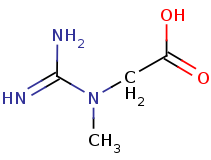
\includegraphics{cr.png}}
	\end{figure}
\end{columns}





\end{frame}

\begin{frame}
\frametitle {Deficienza della guanidinoacetato metiltransferasi (GAMT)}
\framesubtitle {Creatina}
\begin{columns}
	\column{.60\textwidth}
	$Cr + ATP \leftrightharpoons PCr + ADP$ (fosforilazione)
	\column{.40\textwidth}
	\begin{figure}
		\resizebox{!}{0.15\paperheight}{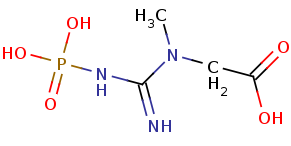
\includegraphics{pcr.png}}
	\end{figure}
	\centering Fosfocreatina (PCr)
	\end{columns}
	
	\begin{columns}
	\column{.60\textwidth}
	$Cr + H_2O \rightarrow Crn$ (degradazione)
	\column{.40\textwidth}
	\begin{figure}
		\resizebox{!}{0.15\paperheight}{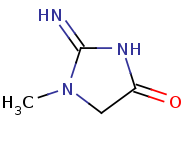
\includegraphics{creatinine.png}}
	\end{figure}
	\centering Creatinina (Crn)
\end{columns}



\end{frame}
\begin{frame}
\frametitle {Deficienza della guanidinoacetato metiltransferasi (GAMT)}
\framesubtitle {Sintesi della creatina}
\begin{columns}
	\column{.60\textwidth}
	$Arg + Gly \xleftrightharpoons{AGAT} Orn + GAA$ (nei reni)
	\column{.40\textwidth}
	\begin{figure}
		\resizebox{!}{0.15\paperheight}{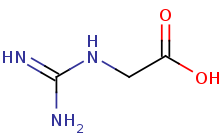
\includegraphics{guanidinoacetate.png}}
	\end{figure}
	\centering Acido guanidinoacetico (GAA)
\end{columns}

\visible<2->{
\begin{columns}
	\column{.60\textwidth}
	$GAA + SAM \xleftrightharpoons{GAMT} Cr + SAH$ (nel fegato)
	\column{.40\textwidth}
	\begin{figure}
		\resizebox{!}{0.15\paperheight}{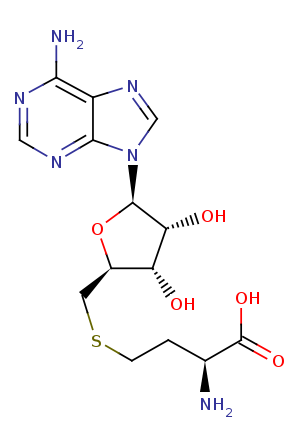
\includegraphics{sadenosylhomocysteine.png}}
	\end{figure}
	\centering S-adenosil omocisteina (SAH)
\end{columns}}
\end{frame}

\begin{frame}
\frametitle {Deficienza della guanidinoacetato metiltransferasi (GAMT)}
\framesubtitle {Sintesi dell'S-adenosil metionina}
\begin{columns}
	\column{.60\textwidth}
	$Met + ATP \xrightarrow{SAMS} SAM + P_i + PP_i$
	\column{.40\textwidth}
	\begin{figure}
		\resizebox{!}{0.45\paperheight}{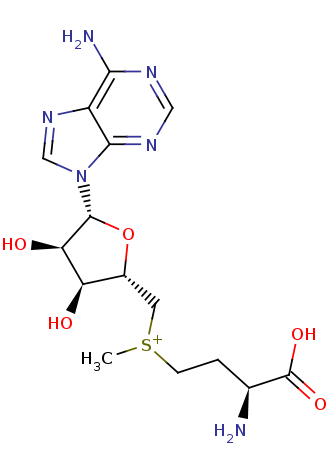
\includegraphics{sadenosylmethionine.png}}
	\end{figure}
	\centering S-adenosil metionina (SAM)
\end{columns}


\end{frame}

\begin{frame}
\frametitle {Deficienza della guanidinoacetato metiltransferasi (GAMT)}
\framesubtitle {Generalit\`a}

I difetti metabolici della creatina possono colpire gli enzimi AGAT, GAMT e di trasporto (SLC6A8 e OCT3)

La deficienza GAMT \`e la pi\`u grave perch\'e il \alert{GAA si accumula}, non essendo utilizzato da altre vie

\begin{itemize}
	\item Bassi livelli di Cr causano deficit cognitivi e di sviluppo, e la sovraespressione dei geni mitocondriali per i \emph{Complessi I, III e V}
	\item Elevati livelli di GAA sono neurotossici per antagonismo con il recettore $GABA_A$
\end{itemize}

\end{frame}

\begin{frame}
\frametitle {Deficienza della guanidinoacetato metiltransferasi (GAMT)}
\framesubtitle {Sintomi}
\begin{columns}[t]
\column{.45\textwidth}
\begin{block}{Eccesso di GAA}
\begin{itemize}
	\item Epilessia
	\item Iperattivit\`a di globo pallido, campo H di Forel, sostanza nera e corteccia
	\item Disturbi extrapiramidali
\end{itemize}
\end{block}

\column{.45\textwidth}
\begin{block}{Carenza di Cr}
	\begin{itemize}
		\item Ritardo comportamentale
		\item Disabilit\`a intellettuale (domini del linguaggio e del comportamento)
		\invisible{\item aaa}
	\end{itemize}
	\end{block}
\end{columns}

In pazienti gravemente deficienti vengono compromesse le funzionalit\`a intellettuali e l'indipendenza in et\`a adulta

\end{frame}

\begin{frame}
	\frametitle {Deficienza della guanidinoacetato metiltransferasi (GAMT)}
	\framesubtitle {Diagnosi}

\begin{itemize}
	\item Sequenziamento gene gamt (19p13.3)
	\item Tomografia a risonanza magnetica (segnale relativo al globo pallido elevato)
	\item Spettroscopia a risonanza magnetica $^1H$ su urine e liquor (picchi relativi a Cr e Crn ridotti, picco relativo a GAA elevato)
	\item Spettroscopia a risonanza magnetica $^{31}P$ (picco relativo a PCr basso, presenza di picco relativo a PGAA)
	\item Reazione di Sakaguchi (sul campione si formano macchie rosso-arancio per reazione con GAA)
\end{itemize}

Gli esami di screening sono poco diffusi e la patologia viene tipicamente diagnosticata solo dopo la manifestazione dei sintomi

\end{frame}

\begin{frame}
\frametitle {Deficienza della guanidinoacetato metiltransferasi (GAMT)}
\framesubtitle {Terapie}
\begin{itemize}
	\item Integrazione creatina per via orale (durata del trattamento limitata per impedire sottoespressione di SLC6A8) nelle stesse dosi previste per i difetti del ciclo dell'urea (300-800 $mg/kg/die$)
	\item Limitazione della sintesi di guanidinoacetato tramite carenza di arginina (diete ipoproteiche), integrazione di ornitina (spostamento dell'equilibrio verso i reagenti)
\end{itemize}

Durante la terapia, si osserva il recupero dei livelli fisiologici di creatina, ma i danni da guanidinoacetato sul SNC permangono se il trattamento non \`e tempestivo (prenatale o entro i due mesi)

\end{frame}

\begin{frame}
\frametitle {Red Cell Loader}
\framesubtitle {Apparato}
\begin{figure}
	\centerline{\resizebox{!}{.6\paperheight}{\includegraphics{RBC_Loader.png}}}
\end{figure}

\end{frame}

\begin{frame}
\frametitle {Red Cell Loader}
\framesubtitle {Protocollo sperimentale}
\begin{enumerate}
	\item Incapsulamento enzimi e substrati negli RBC tramite RCL
	\item Verifica delle quantit\`a incapsulate tramite cromatografia liquida ad alte prestazioni
	\item Incubazione con metaboliti esterni (tra cui GAA marcato con $^{13}C$), HEPES (tampone) e PIGPA (conservante)
	\item Analisi elettrospray di GAA e Cr marcate, dopo blocco metabolico per essiccazione su cartoncino
\end{enumerate}

\end{frame}

\begin{frame}[fragile]
	\frametitle{Red Cell Loader}
	\framesubtitle{Esperimenti \emph{in vitro}: uptake del guanidinoacetato da parte degli RBC ingegnerizzati}
\begin{columns}
	\column{.45\textwidth}
			\begin{figure}
				\center
				\resizebox{\textwidth}{!}{
					\begin{tikzpicture}
					\begin{axis}[axis lines=middle, xmin=0, xmax=100, ymin=0, ymax=100,samples=100, xtick={5, 15, 30, 60}, xlabel={$t$}, ylabel={$[GAA^*]$}]
					\addplot[
					scatter,
					point meta=explicit symbolic,
					scatter/classes={
						a={mark=o,draw=black},
						b={mark=x, draw=black},
						c={mark=square,draw=black},
						d={mark=triangle,draw=black},
						e={mark=asterisk,draw=black}}
					]
					table [meta=label, col sep=comma, row sep=crcr]{
						x, y, label, err\\
						0, 0, a, 1\\
						5, 0, a, 2\\
						15, 0, a, 3\\
						30, 0, a, 4\\
						60, 0, a, 5\\
					};
					\addplot[
					scatter,
					point meta=explicit symbolic,
					scatter/classes={
						a={mark=o,draw=black},
						b={mark=x, draw=black},
						c={mark=square,draw=black},
						d={mark=triangle,draw=black},
						e={mark=asterisk,draw=black}}
					]
					table [meta=label, col sep=comma, row sep=crcr]{
						x, y, label\\
						0, 0, b\\
						5, 1, b\\
						15, 3, b\\
						30, 5, b\\
						60, 7, b\\
					};
					\addplot[
					scatter,
					point meta=explicit symbolic,
					scatter/classes={
						a={mark=o,draw=black},
						b={mark=x, draw=black},
						c={mark=square,draw=black},
						d={mark=triangle,draw=black},
						e={mark=asterisk,draw=black}}
					]
					table [meta=label, col sep=comma, row sep=crcr]{
						x, y, label\\
						0, 2, c\\
						5, 3, c\\
						15, 7, c\\
						30, 12, c\\
						60, 17, c\\
					};
					\addplot[
					scatter,
					point meta=explicit symbolic,
					scatter/classes={
						a={mark=o,draw=black},
						b={mark=x, draw=black},
						c={mark=square,draw=black},
						d={mark=triangle,draw=black},
						e={mark=asterisk,draw=black}}
					]
					table [meta=label, col sep=comma, row sep=crcr]{
						x, y, label\\
						0, 3, d\\
						5, 7, d\\
						15, 14, d\\
						30, 25, d\\
						60, 38, d\\
					};
					\addplot[
					scatter,
					point meta=explicit symbolic,
					scatter/classes={
						a={mark=o,draw=black},
						b={mark=x, draw=black},
						c={mark=square,draw=black},
						d={mark=triangle,draw=black},
						e={mark=asterisk,draw=black}}
					]
					table [meta=label, col sep=comma, row sep=crcr]{
						x, y, label\\
						0, 5, e\\
						5, 11, e\\
						15, 24, e\\
						30, 41, e\\
						60, 67, e\\
					};
					
					
					
					\legend{$0\mu M$,$10\mu M$,$25\mu M$,$50\mu M$,$100\mu M$};
					
					\end{axis}
					\end{tikzpicture}
				}
			\end{figure}
	
	
	\column{.45\textwidth}
\begin{figure}
	\center
	\resizebox{.9\textwidth}{!}{
		\begin{tikzpicture}
		\begin{axis}[axis lines=middle, xmin=-0.01, xmax=0.1, ymin=-0.5, ymax=5,domain=-0.1:0.5,samples=100, xlabel={$\frac{1}{[S]}$}, ylabel={$\frac{1}{V}$}]
		\addplot[black]{48.9333*x + 0.0853333};
		\addplot[
		scatter,
		only marks,
		point meta=explicit symbolic,
		scatter/classes={
			a={mark=o,draw=black}}
		]
		table [meta=label, col sep=comma, row sep=crcr]{
			x, y, label\\
			0.1, 5, a\\
			0.04, 2, a\\
			0.02, 1, a\\
			0.01, 0.66, a\\
		};
		
		\legend{$y = 48.9\overline{3}x + 0.085\overline{3}$,Doppi reciproci};
		
		\end{axis}
		\end{tikzpicture}
	}
\end{figure}

\end{columns}
	
\end{frame}

\begin{frame}
	\frametitle{Red Cell Loader}
	\framesubtitle{Esperimenti \emph{in vitro}: sintesi di creatina da parte degli RBC ingegnerizzati}
	
	\begin{columns}[t]
		\column{.3\textwidth}
		\begin{block}{RBC non ingegnerizzati \phantom{aaaaaaaaaaaaaaaaaaaaa}}
			\resizebox{\textwidth}{!} {
				\begin{tabular}{| c | c | c |}
					\hline
					Tempo (ore) & $[GAA]\ (\mu M)$ & $[Cr]\ (\mu M)$ \\
					\hline
					0 & 0.13 & 59.80\\
					\hline
					1 & 0.15 & 72.20\\
					\hline
					2 & 0.16 & 75.25\\
					\hline
					3 & 0.20 & 75.86\\
					\hline
					20 & 0.27 & 76.31\\
					\hline
				\end{tabular}
			}
		\end{block}
		\column{.3\textwidth}
		\begin{block}{250 $\mu g/ml$ di GAMT e 25 $\mu M$ di SAM}
			\resizebox{\textwidth}{!} {
				\begin{tabular}{| c | c | c |}
					\hline
					Tempo (ore) & $[GAA]\ (\mu M)$ & $[Cr]\ (\mu M)$ \\
					\hline
					0 & 2.61 & 66.01\\
					\hline
					1 & 3.10 & 61.90\\
					\hline
					2 & 4.62 & 63.37\\
					\hline
					3 & 5.11 & 67.50\\
					\hline
					20 & 5.26 & 59.31\\
					\hline
				\end{tabular}
			}
		\end{block}
		\column{.3\textwidth}
		\begin{block}{250 $\mu g/ml$ di GAMT e 125 $\mu M$ di SAM}
			\resizebox{\textwidth}{!} {
				\begin{tabular}{| c | c | c |}
					\hline
					Tempo (ore) & $[GAA]\ (\mu M)$ & $[Cr]\ (\mu M)$ \\
					\hline
					0 & 7.32 & 66.32\\
					\hline
					1 & 10.52 & 64.55\\
					\hline
					2 & 13.87 & 65.87\\
					\hline
					3 & 12.18 & 61.58\\
					\hline
					20 & 15.13 & 59.88\\
					\hline
				\end{tabular}
			}
		\end{block}
		
	\end{columns}
	
\end{frame}

\section{Analisi formale della deficienza GAMT}

\begin {frame}
\frametitle {Modellazione formale}
\framesubtitle{Dati preliminari}

\alt<1>{
	\begin{align*}
		Arg + Gly &\xrightleftharpoons{AGAT} Orn + GAA\\
		Met + ATP &\xrightarrow{SAMS} SAM\\
		GAA_{fuori} &\overset{\phantom{\xrightarrow{uptake}}}{\xrightleftharpoons{trasporto}} GAA_{dentro}\\
		GAA_{dentro} + SAM &\xrightarrow{GAMT} Cr + SAH
	\end{align*}
	}
	{
		\begin{align}
		{\color{red}\cancel{\color{black}Arg}} + {\color{red}\cancel{\color{black}Gly}}\nonumber &{\color{red}\cancel{\color{black}\xrightleftharpoons{AGAT}}} {\color{red}\cancel{\color{black}Orn}} + GAA\\
		%Arg + Gly &\xrightleftharpoons{AGAT} Orn + GAA\\
		{\color{gray}Met + ATP} &\xrightarrow{SAMS} SAM\label<1->{sams}\\
		GAA_{fuori} &{\color{red}\overset{\xrightarrow{uptake}}{\cancel{\color{black}\xrightleftharpoons{trasporto}}}} GAA_{dentro}\label<1->{uptake}\\
		GAA_{dentro} + SAM &\xrightarrow{GAMT} Cr + SAH\label<1->{gamt}
		\end{align}
		}


\visible<2>{
	\begin{columns}
		\column{.5\textwidth}
		(\ref{sams}) e (\ref{gamt}) hanno cinetica: $V(A, B) = \frac{\frac{V_{max}}{K_{MA} + [A]} \cdot [B]}{\frac{K_i \cdot K_{MA} + K_{MB} \cdot [A]}{K_{MA} + [A]} + [B]}$
		\column{.5\textwidth}
		(\ref{uptake}) ha cinetica: $V(X_{fuori}, X_{dentro}) = V_{uptake} \cdot ([X]_{fuori} - [X]_{dentro})$
	\end{columns}
	}
\end{frame}

\iffalse

\begin {frame}
\frametitle {Modellazione formale}
\framesubtitle{Modello Bio-PEPA: cinetiche}
\begin{align*}
	sams &= \left [10 \cdot \frac{\frac{v\_sams}{km\_sams\_atp + atp} \cdot met}{\frac{ki\_sams\_sam \cdot km\_sams\_atp + km\_sams\_met \cdot atp}{km\_sams\_atp + atp} + met} \right ]\\
	gamt &= \left [10 \cdot \frac{\frac{v\_gamt}{km\_gamt\_sam + \frac{SAM}{10}} \cdot \frac{GAA\_INT}{10}}{\frac{ki\_gamt\_sah \cdot km\_gamt\_sam + km\_gamt\_gaa\_int \cdot \frac{SAM}{10}}{km\_gamt\_sam + \frac{SAM}{10}} + \frac{GAA\_INT}{10}}\right ]\\
	uptake &= \left [v\_uptake \cdot \frac{GAA\_EXT - GAA\_INT}{10} \right ]
\end{align*}
\end{frame}

\fi

\begin {frame}
\frametitle {Modellazione formale}
\framesubtitle{Modello Bio-PEPA: processi}
\begin{align*}
SAM &= sams \uparrow SAM + gamt \downarrow SAM\\
SAH &= gamt \uparrow SAH\\
GAA\_INT &= uptake \uparrow GAA\_INT + gamt \downarrow GAA\_INT\\
GAA\_EXT &= uptake \downarrow GAA\_EXT\\
CR &= gamt \uparrow CR
\end{align*}
\begin{equation*}
	(SAM \underset{gamt}{\bowtie} SAH \underset{gamt}{\bowtie} GAA\_INT \underset{gamt}{\bowtie} CR)\underset{uptake}{\bowtie} GAA\_EXT
\end{equation*}
\end{frame}

\begin {frame}
\frametitle {Modellazione formale}
\framesubtitle{Modello Bio-PEPA: parametri}
{
\begin{columns}[t]
	\column{.3\textwidth}
	\begin{block}
	{Validazione uptake guanidinoacetato}
	\begin{itemize}
		\item GAA esterno: 10, 25, 50, 100 $\mu M$
		\item Nessun'altra specie chimica
		\item Solo uptake (0.02 $\mu M / min$)
		\invisible{\item SAMS nativa (0.033 $\mu M / min$)}
	\end{itemize}
	\end{block}
	\column{.3\textwidth}
	\begin{block}{Validazione dosaggio creatina}
		\begin{itemize}
			\item GAA esterno: 100 $\mu M$
			\item SAM: 3.5 (valore fisiologico), 10, 50 $\mu M$
			\item GAMT assente (controllo) e circa 0.66 $mg/ml$ (33 $\mu M/min$)
			\item SAMS nativa (0.033 $\mu M / min$)
		\end{itemize}
	\end{block}
	\column{.3\textwidth}
	\begin{block}{Previsione nuovi esperimenti}
		\begin{itemize}
			\item GAA esterno: 50 $\mu M$
			\item SAM: 3.5 $\mu M$
			\item 0.3 $mg/ml $ di GAMT  (15 $\mu M/min$)
			\item SAMS nativa (controllo) e di \emph{E.\ coli} (400 $\mu M/min/mg$):  0.05, 0.1, 0.5, 1, 2.5, 5 $mg$
		\end{itemize}
	\end{block}
\end{columns}
}
\end{frame}

\begin {frame}
\frametitle {Modellazione formale}
\framesubtitle{Modelli PRISM}
\begin{figure}
	\centerline{\resizebox{\paperwidth}{!}{\includegraphics{prism.png}}}
\end{figure}
\end{frame}

\begin {frame}
\frametitle {Analisi simulativa}
\framesubtitle{Uptake}
\begin{figure}
	\center
	\resizebox{!}{0.7\paperheight}{
		\begin{tikzpicture}[spy using outlines={rectangle, magnification=3.0}, connect spies]
		\begin{axis}[axis lines=middle, xmin=0, xmax=60, ymin=0, ymax=70,samples=1000, xtick={0,10,...,60}, xlabel={$t~(min)$}, ylabel={$[GAA*]~(\mu M)$}, legend style={font=\tiny},
		x label style={at={(axis description cs:0.5,-0.1)},anchor=north},
		y label style={at={(axis description cs:-0.1,.5)},rotate=90,anchor=south},
		tick label style={font=\tiny},
		label style={font=\tiny},
		legend pos=outer north east,
		legend entries={$10 \mu M$ GAA*, $25 \mu M$ GAA*, $50 \mu M$ GAA*, $100 \mu M$ GAA*, Sperimentali}]
		
		\addplot[
		ultra thin,
		scatter,forget plot,
		point meta=explicit symbolic,
		scatter/classes={
			gaa10={mark=asterisk,draw=black,mark size=2},
			gaa25={mark=pentagon, draw=black,mark size=2},
			gaa50={mark=diamond, draw=black,mark size=2},
			gaa100={mark=o,draw=black,mark size=2},
			uptakeexp={mark=+,draw=black,mark size=2}}
		]
		file{Dati/001-004/001.txt};
		
		\addplot[
		ultra thin,
		scatter,forget plot,
		point meta=explicit symbolic,
		scatter/classes={
			gaa10={mark=asterisk,draw=black,mark size=2},
			gaa25={mark=pentagon, draw=black,mark size=2},
			gaa50={mark=diamond, draw=black,mark size=2},
			gaa100={mark=o,draw=black,mark size=2},
			uptakeexp={mark=+,draw=black,mark size=2}}
		]
		file{Dati/001-004/002.txt};
		
		
		
		\addplot[
		ultra thin,
		scatter,forget plot,
		point meta=explicit symbolic,
		scatter/classes={
			gaa10={mark=asterisk,draw=black,mark size=2},
			gaa25={mark=pentagon, draw=black,mark size=2},
			gaa50={mark=diamond, draw=black,mark size=2},
			gaa100={mark=o,draw=black,mark size=2},
			uptakeexp={mark=+,draw=black,mark size=2}}
		]
		file{Dati/001-004/003.txt};
		
		\addplot[
		ultra thin,
		scatter,forget plot,
		point meta=explicit symbolic,
		scatter/classes={
			gaa10={mark=asterisk,draw=black,mark size=2},
			gaa25={mark=pentagon, draw=black,mark size=2},
			gaa50={mark=diamond, draw=black,mark size=2},
			gaa100={mark=o,draw=black,mark size=2},
			uptakeexp={mark=+,draw=black,mark size=2}}
		]
		file{Dati/001-004/004.txt};
		
		\addplot[
		ultra thin,
		scatter,
		point meta=explicit symbolic,
		only marks,
		forget plot,
		scatter/classes={
			gaa10={mark=asterisk,draw=black,mark size=2},
			gaa25={mark=pentagon, draw=black,mark size=2},
			gaa50={mark=diamond, draw=black,mark size=2},
			gaa100={mark=o,draw=black,mark size=2},
			uptakeexp={mark=+,draw=black,mark size=2}}
		]
		file{Dati/uptake.txt};
		
		\addlegendimage{mark=asterisk}
		\addlegendimage{mark=pentagon}
		\addlegendimage{mark=diamond}
		\addlegendimage{mark=o}
		\addlegendimage{only marks, mark=+}
		
		
		
		\end{axis}
		\end{tikzpicture}
	}
\end{figure}

\end{frame}

\begin {frame}
\frametitle {Analisi simulativa}
\framesubtitle{Dosaggio}
\begin{columns}
	\column{.5\textwidth}
\begin{figure}
	\center
	\resizebox{\textwidth}{!}{
		\begin{tikzpicture}[spy using outlines={rectangle, magnification=3.0}, connect spies]
		\begin{axis}[axis lines=middle, xmin=0, xmax=300, ymin=0, ymax=85,samples=1000, xtick={0,60,...,300}, xlabel={$t~(min)$}, ylabel={$[Gaa_{int}]~(\mu M)$}, legend style={font=\tiny},
		x label style={at={(axis description cs:0.5,-0.1)},anchor=north},
		y label style={at={(axis description cs:-0.1,.5)},rotate=90,anchor=south},
		tick label style={font=\tiny},
		label style={font=\tiny},
		legend pos=outer north east, mark repeat={10}]
		
		\addplot[
		ultra thin,
		scatter,
		point meta=explicit symbolic,
		scatter/classes={
			sam10={mark=asterisk,draw=black,mark size=2},
			sam50={mark=pentagon, draw=black,mark size=2},
			unload={mark=diamond, draw=black,mark size=2}}
		]
		file{Dati/005-007/005-gaa.txt};
		
		
		
		\addplot[
		ultra thin,
		scatter,
		point meta=explicit symbolic,
		scatter/classes={
			sam10={mark=asterisk,draw=black,mark size=2},
			sam50={mark=pentagon, draw=black,mark size=2},
			unload={mark=diamond, draw=black,mark size=2}}
		]
		file{Dati/005-007/006-gaa.txt};
		
		\addplot[
		ultra thin,
		scatter,
		point meta=explicit symbolic,
		scatter/classes={
			sam10={mark=asterisk,draw=black,mark size=2},
			sam50={mark=pentagon, draw=black,mark size=2},
			unload={mark=diamond, draw=black,mark size=2}}
		]
		file{Dati/005-007/007-gaa.txt};
		
		
		\legend{$10 \mu M$ SAM, $50 \mu M$ SAM, Unloaded};
		
		\coordinate (spypoint) at (axis cs:10,65);
		\coordinate (spyviewer) at (axis cs:100,20);
		\end{axis}
		\spy [height=2.5cm, width=3cm,spy connection path={
			\begin{scope}[on background layer]
			\draw (tikzspyonnode.north east) -- (tikzspyinnode.north east);
			\draw (tikzspyonnode.north west) -- (tikzspyinnode.north west);
			\draw (tikzspyonnode.south west) -- (tikzspyinnode.south west);
			\draw (tikzspyonnode.south east) -- (tikzspyinnode.south east);
			\end{scope}
		}] on (spypoint)
		in node [fill=white] at (spyviewer);
		\end{tikzpicture}
	}
\end{figure}
\column{.5\textwidth}
\begin{figure}
	\center
	\resizebox{\textwidth}{!}{
		\begin{tikzpicture}
		\begin{axis}[axis lines=middle, xmin=0, xmax=120, ymin=0, ymax=60,samples=1000, xtick={0,20,...,120}, xlabel={$t~(min)$}, ylabel={$[Cr]~(\mu M)$}, legend style={font=\tiny},
		x label style={at={(axis description cs:0.5,-0.1)},anchor=north},
		y label style={at={(axis description cs:-0.1,.5)},rotate=90,anchor=south},
		tick label style={font=\tiny},
		label style={font=\tiny},
		legend pos=outer north east, mark repeat={3}]
		
		\addplot[
		ultra thin,
		scatter,
		point meta=explicit symbolic,
		scatter/classes={
			sam10={mark=asterisk,draw=black,mark size=2},
			sam50={mark=pentagon, draw=black,mark size=2},
			unload={mark=diamond, draw=black,mark size=2}}
		]
		file{Dati/005-007/005-cr.txt};
		
		
		
		\addplot[
		ultra thin,
		scatter,
		point meta=explicit symbolic,
		scatter/classes={
			sam10={mark=asterisk,draw=black,mark size=2},
			sam50={mark=pentagon, draw=black,mark size=2},
			unload={mark=diamond, draw=black,mark size=2}}
		]
		file{Dati/005-007/006-cr.txt};
		
		\addplot[
		ultra thin,
		scatter,
		point meta=explicit symbolic,
		scatter/classes={
			sam10={mark=asterisk,draw=black,mark size=2},
			sam50={mark=pentagon, draw=black,mark size=2},
			unload={mark=diamond, draw=black,mark size=2}}
		]
		file{Dati/005-007/007-cr.txt};
		
		
		\legend{$10 \mu M$ SAM, $50 \mu M$ SAM, Unloaded};
		
		\end{axis}
		\end{tikzpicture}
	}
\end{figure}
\end{columns}

\end{frame}

\begin {frame}
\frametitle {Analisi simulativa}
\framesubtitle{Nuovi esperimenti}
\begin{columns}
	\column{.5\textwidth}
\begin{figure}
	\center
	\resizebox{\textwidth}{!}{
		\begin{tikzpicture}[spy using outlines={rectangle, magnification=3.0}, connect spies]
		\begin{axis}[axis lines=middle, xmin=0, xmax=600, ymin=0, ymax=55,samples=1000, xtick={0,60,...,600}, xlabel={$t~(min)$}, ylabel={$[Cr]~(\mu M)$}, legend style={font=\tiny},
		x label style={at={(axis description cs:0.5,-0.1)},anchor=north},
		y label style={at={(axis description cs:-0.1,.5)},rotate=90,anchor=south},
		tick label style={font=\tiny},
		label style={font=\tiny},
		legend pos=outer north east, mark repeat={3}]
		
		\addplot[
		ultra thin,
		scatter,
		point meta=explicit symbolic,
		scatter/classes={
			emat={mark=asterisk,draw=black,mark size=2},
			eco005={mark=pentagon, draw=black,mark size=2},
			eco01={mark=diamond, draw=black,mark size=2},
			eco05={mark=o,draw=black,mark size=2},
			eco1={mark=x, draw=black,mark size=2},
			eco25={mark=square,draw=black,mark size=2},
			eco5={mark=triangle,draw=black,mark size=2}}
		]
		file{Dati/008-014/008-cr.txt};
		
		\addplot[
		ultra thin,
		scatter,
		point meta=explicit symbolic,
		scatter/classes={
			emat={mark=asterisk,draw=black,mark size=2},
			eco005={mark=pentagon, draw=black,mark size=2},
			eco01={mark=diamond, draw=black,mark size=2},
			eco05={mark=o,draw=black,mark size=2},
			eco1={mark=x, draw=black,mark size=2},
			eco25={mark=square,draw=black,mark size=2},
			eco5={mark=triangle,draw=black,mark size=2}}
		]
		file{Dati/008-014/009-cr.txt};
		
		
		
		\addplot[
		ultra thin,
		scatter,
		point meta=explicit symbolic,
		scatter/classes={
			emat={mark=asterisk,draw=black,mark size=2},
			eco005={mark=pentagon, draw=black,mark size=2},
			eco01={mark=diamond, draw=black,mark size=2},
			eco05={mark=o,draw=black,mark size=2},
			eco1={mark=x, draw=black,mark size=2},
			eco25={mark=square,draw=black,mark size=2},
			eco5={mark=triangle,draw=black,mark size=2}}
		]
		file{Dati/008-014/010-cr.txt};
		
		\addplot[
		ultra thin,
		scatter,
		point meta=explicit symbolic,
		scatter/classes={
			emat={mark=asterisk,draw=black,mark size=2},
			eco005={mark=pentagon, draw=black,mark size=2},
			eco01={mark=diamond, draw=black,mark size=2},
			eco05={mark=o,draw=black,mark size=2},
			eco1={mark=x, draw=black,mark size=2},
			eco25={mark=square,draw=black,mark size=2},
			eco5={mark=tria del modellongle,draw=black,mark size=2}}
		]
		file{Dati/008-014/011-cr.txt};
		
		\addplot[
		ultra thin,
		scatter,
		point meta=explicit symbolic,
		scatter/classes={
			emat={mark=asterisk,draw=black,mark size=2},
			eco005={mark=pentagon, draw=black,mark size=2},
			eco01={mark=diamond, draw=black,mark size=2},
			eco05={mark=o,draw=black,mark size=2},
			eco1={mark=x, draw=black,mark size=2},
			eco25={mark=square,draw=black,mark size=2},
			eco5={mark=triangle,draw=black,mark size=2}}
		]
		file{Dati/008-014/012-cr.txt};
		
		\addplot[
		ultra thin,
		scatter,
		point meta=explicit symbolic,
		scatter/classes={
			emat={mark=asterisk,draw=black,mark size=2},
			eco005={mark=pentagon, draw=black,mark size=2},
			eco01={mark=diamond, draw=black,mark size=2},
			eco05={mark=o,draw=black,mark size=2},
			eco1={mark=x, draw=black,mark size=2},
			eco25={mark=square,draw=black,mark size=2},
			eco5={mark=triangle,draw=black,mark size=2}}
		]
		file{Dati/008-014/013-cr.txt};
		
		
		\legend{H. sapiens, $0.05mg$, $0.1mg$, $0.5mg$, $1.0mg$, $2.5mg$};
		
		\coordinate (spypoint) at (axis cs:30,5);
		\coordinate (spyviewer) at (axis cs:120,50);
		\end{axis}
		\spy [height=1.5cm, width=2cm,spy connection path={
			\begin{scope}[on background layer]
			\draw (tikzspyonnode.north east) -- (tikzspyinnode.north east);
			\draw (tikzspyonnode.north west) -- (tikzspyinnode.north west);
			\draw (tikzspyonnode.south west) -- (tikzspyinnode.south west);
			\draw (tikzspyonnode.south east) -- (tikzspyinnode.south east);
			\end{scope}
		}] on (spypoint)
		in node [fill=white] at (spyviewer);
		\end{tikzpicture}
	}
\end{figure}
\column{.5\textwidth}
\begin{figure}
	\center
	\resizebox{\textwidth}{!}{
		\begin{tikzpicture}
		\begin{axis}[axis lines=middle, xmin=0, xmax=600, ymin=0, ymax=27
		,samples=1000, xtick={0,60,...,600}, xlabel={$t~(min)$}, ylabel={$[GAA_{int}]~(\mu M)$}, legend style={font=\tiny},
		x label style={at={(axis description cs:0.5,-0.1)},anchor=north},
		y label style={at={(axis description cs:-0.1,.5)},rotate=90,anchor=south},
		tick label style={font=\tiny},
		label style={font=\tiny},
		legend pos=outer north east,mark repeat={3}]
		
		\addplot[
		ultra thin,
		scatter,
		point meta=explicit symbolic,
		scatter/classes={
			emat={mark=asterisk,draw=black,mark size=2},
			eco005={mark=pentagon, draw=black,mark size=2},
			eco01={mark=diamond, draw=black,mark size=2},
			eco05={mark=o,draw=black,mark size=2},
			eco1={mark=x, draw=black,mark size=2},
			eco25={mark=square,draw=black,mark size=2},
			eco5={mark=triangle,draw=black,mark size=2}}
		]
		file{Dati/008-014/008-gaa_int.txt};
		
		\addplot[
		ultra thin,
		scatter,
		point meta=explicit symbolic,
		scatter/classes={
			emat={mark=asterisk,draw=black,mark size=2},
			eco005={mark=pentagon, draw=black,mark size=2},
			eco01={mark=diamond, draw=black,mark size=2},
			eco05={mark=o,draw=black,mark size=2},
			eco1={mark=x, draw=black,mark size=2},
			eco25={mark=square,draw=black,mark size=2},
			eco5={mark=triangle,draw=black,mark size=2}}
		]
		file{Dati/008-014/009-gaa_int.txt};
		
		\addplot[
		ultra thin,
		scatter,
		point meta=explicit symbolic,
		scatter/classes={
			emat={mark=asterisk,draw=black,mark size=2},
			eco005={mark=pentagon, draw=black,mark size=2},
			eco01={mark=diamond, draw=black,mark size=2},
			eco05={mark=o,draw=black,mark size=2},
			eco1={mark=x, draw=black,mark size=2},
			eco25={mark=square,draw=black,mark size=2},
			eco5={mark=triangle,draw=black,mark size=2}}
		]
		file{Dati/008-014/010-gaa_int.txt};
		
		\addplot[
		ultra thin,
		scatter,
		point meta=explicit symbolic,
		scatter/classes={
			emat={mark=asterisk,draw=black,mark size=2},
			eco005={mark=pentagon, draw=black,mark size=2},
			eco01={mark=diamond, draw=black,mark size=2},
			eco05={mark=o,draw=black,mark size=2},
			eco1={mark=x, draw=black,mark size=2},
			eco25={mark=square,draw=black,mark size=2},
			eco5={mark=triangle,draw=black,mark size=2}}
		]
		file{Dati/008-014/011-gaa_int.txt};
		
		\addplot[
		ultra thin,
		scatter,
		point meta=explicit symbolic,
		scatter/classes={
			emat={mark=asterisk,draw=black,mark size=2},
			eco005={mark=pentagon, draw=black,mark size=2},
			eco01={mark=diamond, draw=black,mark size=2},
			eco05={mark=o,draw=black,mark size=2},
			eco1={mark=x, draw=black,mark size=2},
			eco25={mark=square,draw=black,mark size=2},
			eco5={mark=triangle,draw=black,mark size=2}}
		]
		file{Dati/008-014/012-gaa_int.txt};
		
		\addplot[
		ultra thin,
		scatter,
		point meta=explicit symbolic,
		scatter/classes={
			emat={mark=asterisk,draw=black,mark size=2},
			eco005={mark=pentagon, draw=black,mark size=2},
			eco01={mark=diamond, draw=black,mark size=2},
			eco05={mark=o,draw=black,mark size=2},
			eco1={mark=x, draw=black,mark size=2},
			eco25={mark=square,draw=black,mark size=2},
			eco5={mark=triangle,draw=black,mark size=2}}
		]
		file{Dati/008-014/013-gaa_int.txt};
		
		
		
		\legend{H. sapiens, $0.05mg$, $0.1mg$, $0.5mg$, $1.0mg$, $2.5mg$};
		
		\end{axis}
		\end{tikzpicture}
	}
\end{figure}
\end{columns}

\end{frame}

\begin {frame}
\frametitle {Verifica formale}
\framesubtitle{Nuovi esperimenti}

\centering
\begin{tabular}{|c|c|c|}
	\hline
Propriet\`a & Esito & Tempo impiegato\\
\hline\hline
$\mathbb{P}_{=?} [ \mathcal{F}^{ \leq 600 min} \_SAM\_at\_maximum ]$ & 0.99999 & 67152.519 secondi\\
\hline
$\mathbb{P}_{=?} [ \mathcal{F}^{[600 min,600 min]} \_GAA\_INT\_at\_maximum ]$ & 0 & 65071.259 secondi \\
\hline
$\mathbb{R}_{\{\_UM\_SAM\}=?} [ \mathcal{I}=600 min ]$ & 58.49219 $\mu M$ & 65468.829 secondi \\
\hline
$\mathbb{R}_{\{\_UM\_SAH\}=?} [ \mathcal{I}=600 min ]$ & 34.57216 $\mu M$ & 66046.642 secondi \\
\hline
$\mathbb{R}_{\{\_UM\_GAA\_INT\}=?} [ \mathcal{I}=600 min ]$ & 9.61583 $\mu M$ & 65381.08 secondi \\
\hline
$\mathbb{R}_{\{\_UM\_GAA\_EXT\}=?} [ \mathcal{I}=600 min ]$ & 10.812000 $\mu M$ & 65364.411 secondi \\
\hline
$\mathbb{R}_{\{\_UM\_CR\}=?} [ \mathcal{I}=600 min ]$ & 33.27216 $\mu M$ & 65343.736 secondi \\
\hline
$\mathbb{R}_{\{\_sams\}=?} [ \mathcal{C} \leq 600 min ]$ & 882.566 (simulazione) & N/A \\
\hline
$\mathbb{R}_{\{\_gamt\}=?} [ \mathcal{C} \leq 600 min ]$ & 332.971 (simulazione) & N/A \\
\hline
$\mathbb{R}_{\{\_uptake\}=?} [ \mathcal{C} \leq 600 min ]$ & 392.443 (simulazione) & N/A\\
\hline
$\mathbb{P}_{=?} [\mathcal{F} \mathcal{G} \_SAM \leq 10 \mu M]$ & 0 & 292.23 secondi \\
\hline
\end{tabular}

\end{frame}
\section {Conclusione}

\begin {frame}
\frametitle {Conclusioni}
\framesubtitle{Pro e contro}
\begin{columns}[t]
	\column{.45\textwidth}
	\begin{block}
		{Analisi simulativa}
		\setbeamercolor{itemize item}{fg=green}
		\begin{itemize}
			\item [+] ampia diffusione
			\item [+] rapido (ma dipende dalla durata della simulazione)
			\item [+] richiede poche risorse
		\end{itemize}
		\setbeamercolor{itemize item}{fg=red}
		\begin{itemize}
			\item [-] non esaustivo
			\item [-] accumula errori
			\item [-] necessaria la media di pi\`u simulazioni \phantom{aaaaaaaaa}
		\end{itemize}
	\end{block}
	\column{.45\textwidth}
	\begin{block}{Model checking}
		\setbeamercolor{itemize item}{fg=green}
		\begin{itemize}
			\item [+] esaustivo
			\item [+] esente da errori di approssimazione
			\item [+] indipendente dai limiti temporali imposti
		\end{itemize}
		\setbeamercolor{itemize item}{fg=red}
		\begin{itemize}
			\item [-] difficile da utilizzare
			\item [-] lento e computazionalmente complesso
			\item [-] avido di risorse
		\end{itemize}
	\end{block}
\end{columns}

\end{frame}

\begin {frame}
\frametitle {Conclusioni}
\framesubtitle{Sviluppi futuri}
\begin{enumerate}
	\item Verifica \emph{in vitro} della fedelt\`a delle analisi \emph{in silico}
	\item Aggiunta di interazioni complesse \emph{in vivo}
	\item Model checking di aspetti che emergeranno eventualmente da nuovi esperimenti
	\item Semplificazione del modello per verificare altre propriet\`a (e.g. $\mathbb{P}_{=?} [\mathcal{G} (\_SAM = 0 \rightarrow \mathcal{F}^{\leq T} \_SAM > soglia)]$, $\mathbb{P}_{=?} [\mathcal{F}\mathcal{G}^{\leq T} \_GAA\_INT > soglia]$)
\end{enumerate}

\end{frame}


\end{document}